\section{Results and Discussion}
\subsection{Link-Risk Prediction Performance}
The ANN predictor gives an overall RMSE of 4.592 dB, MAE of 3.865 dB, and Pearson correlation of 0.810. Weather-wise RMSE is 4.494 dB for clear, 4.608 dB for rainy, and 4.919 dB for rain-hot. This supports the use of weather-wise calibration, but it also shows that harsh-weather prediction remains imperfect.

\subsection{Main Result Against External Baselines}
Table~\ref{tab:main_results} gives the combined-stress paper-lock results. \pclr\ has objective 0.684, while Reactive-3C has 0.731. This is a 6.47\% objective improvement over Reactive-3C. \pclr\ reduces average delay by 0.61\%, p95 delay by 2.14\%, handovers by 24.52\%, and outage by 9.14\%. The corrected p-values are 0.00653 for average delay, $7.60\times10^{-7}$ for p95 delay, $2.53\times10^{-7}$ for handovers, and 0.0285 for outage. These are treated as statistically reliable.

\pclr\ does not dominate all metrics. Compared with Reactive-3C, it increases energy consumption by 0.72\%, reduces useful cache hit ratio by 1.05\%, and increases drop rate by 0.53\%. The energy difference is Holm-corrected significant, but it is a worsening for \pclr. The useful cache and drop-rate differences are not corrected significant in the Reactive-3C comparison.

\begin{table*}[!t]
\centering
\caption{Combined-stress paper-lock results on blind seeds 4001--4080. Energy is in kJ. Cache, outage, and drop are in percent. Oracle methods are upper bounds and excluded from practical ranking.}
\label{tab:main_results}
\tiny
\begin{tabular}{lccccccccc}
\toprule
Method & Avg Delay & p95 Delay & Energy & Handovers/100 & Useful Cache & Outage & Drop & Throughput & Objective \\
\midrule
Random & 6.32 $\pm$ 0.05 & \textbf{7.70 $\pm$ 0.08} & 20.19 $\pm$ 0.20 & 58.15 $\pm$ 0.48 & 0.00 $\pm$ 0.00 & 1.31 $\pm$ 0.10 & 41.55 $\pm$ 1.91 & 598.3 $\pm$ 4.7 & 2.995 $\pm$ 0.025 \\
Nearest & 6.52 $\pm$ 0.04 & 7.89 $\pm$ 0.08 & 19.50 $\pm$ 0.27 & \textbf{1.33 $\pm$ 0.16} & 0.00 $\pm$ 0.00 & \textbf{0.23 $\pm$ 0.02} & 42.17 $\pm$ 1.82 & 591.6 $\pm$ 8.8 & 0.732 $\pm$ 0.012 \\
RateMax & 6.40 $\pm$ 0.04 & 7.72 $\pm$ 0.07 & 20.19 $\pm$ 0.20 & 34.40 $\pm$ 0.60 & 0.00 $\pm$ 0.00 & 0.82 $\pm$ 0.06 & 43.08 $\pm$ 1.94 & 583.5 $\pm$ 4.7 & 2.085 $\pm$ 0.024 \\
MUCCO-like & 6.28 $\pm$ 0.07 & 8.06 $\pm$ 0.09 & \textbf{16.57 $\pm$ 0.15} & 17.49 $\pm$ 0.54 & 26.63 $\pm$ 0.62 & 0.79 $\pm$ 0.07 & \textbf{37.29 $\pm$ 1.93} & \textbf{653.4 $\pm$ 5.7} & 1.228 $\pm$ 0.024 \\
Reactive-3C & 6.26 $\pm$ 0.07 & 8.02 $\pm$ 0.10 & 16.69 $\pm$ 0.14 & 3.86 $\pm$ 0.22 & \textbf{27.71 $\pm$ 0.60} & 0.96 $\pm$ 0.07 & 37.98 $\pm$ 1.91 & 643.8 $\pm$ 5.7 & 0.731 $\pm$ 0.018 \\
P3C-LR Core & \textbf{6.22 $\pm$ 0.07} & 7.85 $\pm$ 0.10 & 16.81 $\pm$ 0.16 & 2.92 $\pm$ 0.22 & 27.42 $\pm$ 0.68 & 0.88 $\pm$ 0.06 & 38.18 $\pm$ 1.84 & 643.4 $\pm$ 6.5 & 0.684 $\pm$ 0.016 \\
P3C-SR & 6.24 $\pm$ 0.07 & 7.87 $\pm$ 0.10 & 16.89 $\pm$ 0.15 & 2.77 $\pm$ 0.19 & 27.45 $\pm$ 0.63 & 0.81 $\pm$ 0.05 & 37.82 $\pm$ 1.90 & 647.3 $\pm$ 6.2 & \textbf{0.671 $\pm$ 0.016} \\
ET-P3C & 6.22 $\pm$ 0.07 & 7.84 $\pm$ 0.10 & 16.82 $\pm$ 0.15 & 2.76 $\pm$ 0.19 & 27.44 $\pm$ 0.67 & 0.88 $\pm$ 0.06 & 38.13 $\pm$ 1.83 & 643.4 $\pm$ 6.3 & 0.680 $\pm$ 0.017 \\
\textit{OracleLink Upper Bound} & \textit{6.21 $\pm$ 0.07} & \textit{7.85 $\pm$ 0.10} & \textit{16.82 $\pm$ 0.15} & \textit{3.95 $\pm$ 0.25} & \textit{27.58 $\pm$ 0.62} & \textit{0.87 $\pm$ 0.06} & \textit{38.11 $\pm$ 1.89} & \textit{643.9 $\pm$ 6.1} & \textit{0.720 $\pm$ 0.019} \\
\textit{OracleSelector Upper Bound} & \textit{6.26 $\pm$ 0.06} & \textit{7.85 $\pm$ 0.09} & \textit{17.96 $\pm$ 0.17} & \textit{11.20 $\pm$ 0.74} & \textit{19.99 $\pm$ 0.83} & \textit{0.73 $\pm$ 0.05} & \textit{39.33 $\pm$ 2.00} & \textit{658.4 $\pm$ 4.1} & \textit{1.020 $\pm$ 0.032} \\
\bottomrule
\end{tabular}
\end{table*}

\begin{table*}[!t]
\centering
\caption{Percentage change of P3C-LR Core against external baselines under combined stress. Positive values favour P3C-LR Core; negative values show worsening.}
\label{tab:external_baseline}
\scriptsize
\begin{tabular}{lccccccccc}
\toprule
Baseline & Avg Delay & p95 Delay & Energy & Handovers & Useful Cache & Outage & Drop & Throughput & Objective \\
\midrule
Reactive-3C & +0.61\% & +2.14\% & -0.72\% & +24.52\% & -1.05\% & +9.14\% & -0.53\% & -0.06\% & +6.47\% \\
MUCCO-like & +1.01\% & +2.56\% & -1.44\% & +83.33\% & +2.96\% & -11.40\% & -2.38\% & -1.54\% & +44.32\% \\
RateMax & +2.89\% & -1.67\% & +16.77\% & +91.52\% & n/a & -6.22\% & +11.37\% & +10.27\% & +67.20\% \\
\bottomrule
\end{tabular}
\end{table*}


\subsection{Comparison with MUCCO-like and RateMax}
Compared with MUCCO-like, \pclr\ improves the objective by 44.32\%, average delay by 1.01\%, p95 delay by 2.56\%, handovers by 83.33\%, and useful cache hit ratio by 2.96\%. It uses 1.44\% more energy, has 11.40\% higher outage, and has 2.38\% higher drop rate. This shows that MUCCO-like remains strong on energy and drop rate, but it has much higher handover cost in this dynamic setting.

Compared with RateMax, \pclr\ improves the objective by 67.20\%, average delay by 2.89\%, energy by 16.77\%, handovers by 91.52\%, drop rate by 11.37\%, and throughput by 10.27\%. However, RateMax has 1.67\% better p95 delay and 6.22\% lower outage in the combined-stress table. Thus, rate maximization alone is not enough for the aggregate energy-latency-handover objective, but it can still help some tail or outage metrics.

\subsection{Internal Variant Analysis}
Table~\ref{tab:internal_variant} compares \pclr, \psr, and \etp. \psr\ achieves the best aggregate non-oracle objective, 0.671, and is therefore the strongest overall non-oracle method by the paper objective. \pclr\ is the lightweight core and ranks first against external baselines. \etp\ is close to both methods but does not provide reliable additional gain. The manuscript therefore presents \pchorch\ as a framework containing the practical core and the stability-regularized internal variant.

\begin{table*}[!t]
\centering
\caption{Internal P3C-Orch variant comparison under combined stress. Energy is in kJ and ratio metrics are in percent.}
\label{tab:internal_variant}
\scriptsize
\begin{tabular}{lccccccccc}
\toprule
Variant & Avg Delay & p95 Delay & Energy & Handovers & Useful Cache & Outage & Drop & Throughput & Objective \\
\midrule
P3C-LR Core & 6.22 & 7.85 & 16.81 & 2.92 & 27.42 & 0.88 & 38.18 & 643.4 & 0.684 \\
P3C-SR & 6.24 & 7.87 & 16.89 & 2.77 & 27.45 & 0.81 & 37.82 & 647.3 & 0.671 \\
ET-P3C & 6.22 & 7.84 & 16.82 & 2.76 & 27.44 & 0.88 & 38.13 & 643.4 & 0.680 \\
\bottomrule
\end{tabular}
\end{table*}


\subsection{Regime-Wise Behaviour}
Fig.~\ref{fig:delay_cdf} shows the delay CDF under the paper-lock evaluation. Figs.~\ref{fig:energy_regime} and~\ref{fig:handover_regime} show energy and handover behaviour by regime. \pclr\ is useful when link risk and handover decisions matter, but the gains vary by regime. The regime-wise table is generated in \texttt{tables/regime\_results.tex} and retained for detailed checking.

\begin{figure}[!t]
\centering
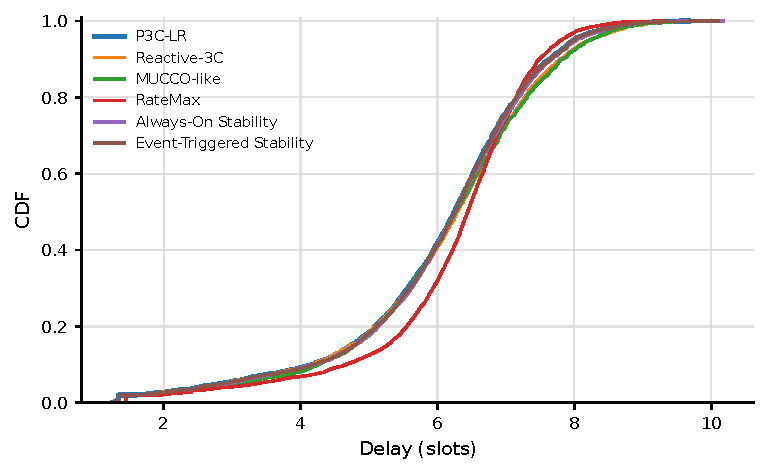
\includegraphics[width=\columnwidth]{figs/delay_cdf_paperlock.pdf}
\caption{Delay CDF for the main methods. The figure compares external baselines and internal variants under the final paper-lock evaluation.}
\label{fig:delay_cdf}
\end{figure}

\begin{figure}[!t]
\centering
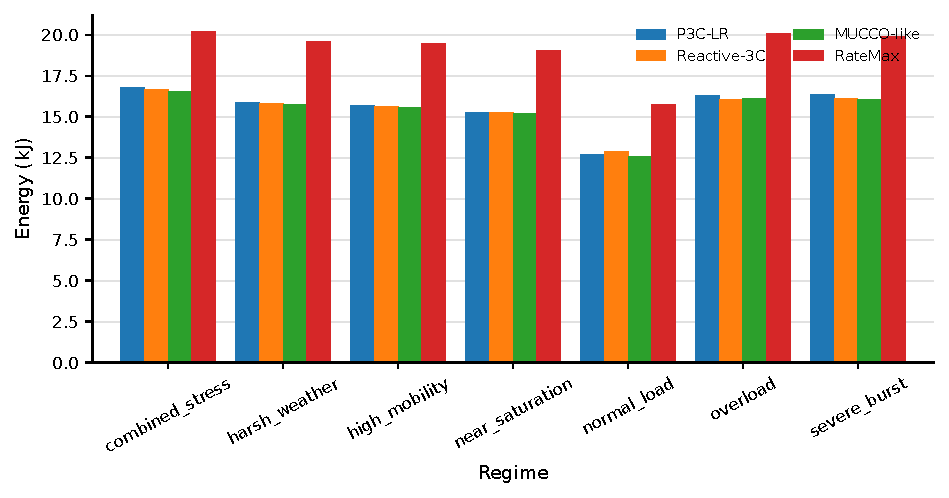
\includegraphics[width=\columnwidth]{figs/energy_by_regime_paperlock.pdf}
\caption{Energy consumption by regime. \pclr\ improves the aggregate objective against external baselines but has a small energy cost compared with Reactive-3C under combined stress.}
\label{fig:energy_regime}
\end{figure}

\begin{figure}[!t]
\centering
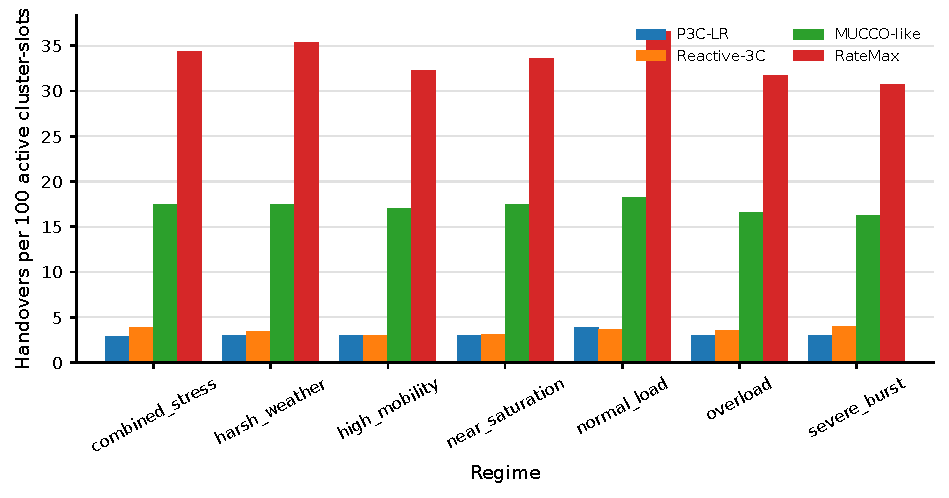
\includegraphics[width=\columnwidth]{figs/handover_by_regime_paperlock.pdf}
\caption{Handovers per 100 active cluster-slots by regime. Mobility-aware dwell control reduces unnecessary switching compared with rate-centric and caching-centric baselines.}
\label{fig:handover_regime}
\end{figure}

\subsection{Cache, Weather, and Oracle Gap}
Fig.~\ref{fig:cache_breakdown} shows cache-hit behaviour. Cache value helps when a hit reduces delay or energy, but \pclr\ can lose useful cache hit ratio against Reactive-3C because the scheduler also gives weight to outage and dwell. Fig.~\ref{fig:outage_weather} shows outage by weather. Fig.~\ref{fig:oracle_gap} shows the gap to upper bounds. Oracle methods are not practical baselines and are used only to show remaining headroom.

\begin{figure}[!t]
\centering
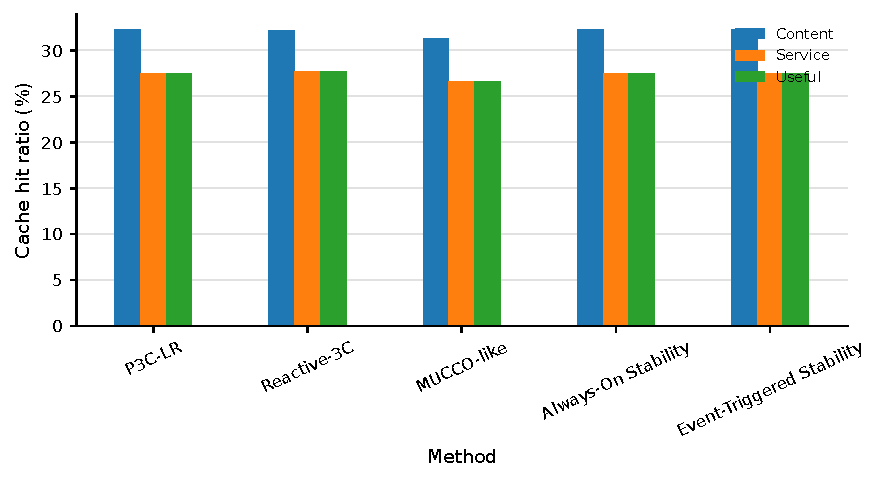
\includegraphics[width=\columnwidth]{figs/cache_hit_breakdown_paperlock.pdf}
\caption{Cache hit breakdown for the main methods. The figure separates cache effects instead of treating every cached file as useful.}
\label{fig:cache_breakdown}
\end{figure}

\begin{figure}[!t]
\centering
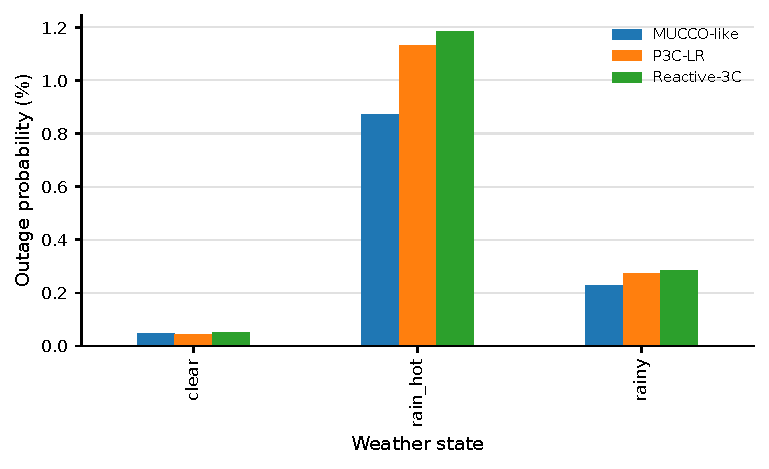
\includegraphics[width=\columnwidth]{figs/outage_by_weather_paperlock.pdf}
\caption{Outage behaviour by weather. Harsh weather increases link risk, which motivates prediction and calibration.}
\label{fig:outage_weather}
\end{figure}

\begin{figure}[!t]
\centering
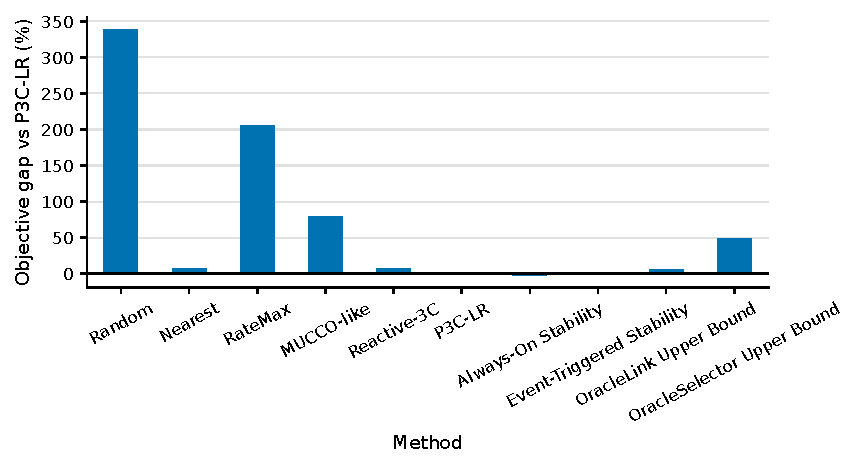
\includegraphics[width=\columnwidth]{figs/oracle_gap_paperlock.pdf}
\caption{Oracle gap under the paper-lock objective. OracleLink and OracleSelector are upper bounds and are excluded from practical ranking.}
\label{fig:oracle_gap}
\end{figure}

\subsection{Statistical Significance}
Only Holm-corrected significant results are treated as statistically reliable. Table~\ref{tab:significance} reports the corrected p-values. The main supported improvements over Reactive-3C are average delay, p95 delay, handovers, and outage. Energy is also corrected significant, but it is worse for \pclr. Hence, the main claim is a latency-handover-outage tradeoff, not universal dominance.

\begin{table*}[!t]
\centering
\caption{Holm-corrected Wilcoxon tests comparing P3C-LR Core with each baseline under combined stress. The Yes column only marks corrected $p<0.05$ and does not imply that the direction favours P3C-LR Core.}
\label{tab:significance}
\tiny
\begin{tabular}{llccc}
\toprule
Baseline & Metric & Corrected $p$ & Effect $d_z$ & $p<0.05$ \\
\midrule
Reactive-3C & Avg delay & 0.00653 & -0.417 & Yes \\
Reactive-3C & p95 delay & 7.6e-07 & -0.719 & Yes \\
Reactive-3C & Energy & 0.0211 & +0.404 & Yes \\
Reactive-3C & Handovers & 2.53e-07 & -0.780 & Yes \\
Reactive-3C & Useful cache & 1 & -0.161 & No \\
Reactive-3C & Outage & 0.0285 & -0.382 & Yes \\
Reactive-3C & Drop rate & 1 & +0.227 & No \\
Reactive-3C & Throughput & 1 & -0.043 & No \\
MUCCO-like & Avg delay & 5.69e-06 & -0.701 & Yes \\
MUCCO-like & p95 delay & 3.54e-07 & -0.761 & Yes \\
MUCCO-like & Energy & 5.97e-07 & +0.778 & Yes \\
MUCCO-like & Handovers & 3.14e-13 & -5.492 & Yes \\
MUCCO-like & Useful cache & 0.00178 & +0.426 & Yes \\
MUCCO-like & Outage & 0.0258 & +0.304 & Yes \\
MUCCO-like & Drop rate & 3.12e-09 & +0.918 & Yes \\
MUCCO-like & Throughput & 4.03e-09 & -0.945 & Yes \\
RateMax & Avg delay & 8.04e-09 & -0.891 & Yes \\
RateMax & p95 delay & 0.0276 & +0.412 & Yes \\
RateMax & Energy & 3.14e-13 & -7.536 & Yes \\
RateMax & Handovers & 3.14e-13 & -10.877 & Yes \\
RateMax & Useful cache & 3.14e-13 & +8.806 & Yes \\
RateMax & Outage & 0.202 & +0.210 & No \\
RateMax & Drop rate & 3.14e-13 & -3.375 & Yes \\
RateMax & Throughput & 3.14e-13 & +2.738 & Yes \\
P3C-SR & Avg delay & 0.623 & -0.246 & No \\
P3C-SR & p95 delay & 1 & -0.125 & No \\
P3C-SR & Energy & 0.0558 & -0.368 & No \\
P3C-SR & Handovers & 1 & +0.145 & No \\
P3C-SR & Useful cache & 1 & -0.020 & No \\
P3C-SR & Outage & 0.024 & +0.344 & Yes \\
P3C-SR & Drop rate & 0.0313 & +0.368 & Yes \\
P3C-SR & Throughput & 0.00644 & -0.477 & Yes \\
ET-P3C & Avg delay & 1 & -0.095 & No \\
ET-P3C & p95 delay & 1 & +0.034 & No \\
ET-P3C & Energy & 1 & -0.065 & No \\
ET-P3C & Handovers & 1 & +0.179 & No \\
ET-P3C & Useful cache & 1 & -0.017 & No \\
ET-P3C & Outage & 1 & -0.013 & No \\
ET-P3C & Drop rate & 1 & +0.077 & No \\
ET-P3C & Throughput & 1 & -0.001 & No \\
\bottomrule
\end{tabular}
\end{table*}


\subsection{Main Observations}
\begin{itemize}
    \item Link-risk prediction is useful when weather and mobility change the service quality.
    \item Mobility-aware dwell control reduces unnecessary handovers.
    \item Cache value helps when cached content reduces delay or energy, but cache hit ratio can drop when link-risk and dwell terms dominate.
    \item \psr\ gives the best aggregate non-oracle objective, but it does not remove all tradeoffs.
    \item \etp\ did not give reliable additional gain in this implementation.
\end{itemize}
